\KOMAoptions{paper=A3}
\recalctypearea
\subsection{Recaman's Sequence}{\label{pp:recamanssequence}}
The Recaman's sequence is defined as below:
\begin{itemize}
	\item $r_0 = 0$
	\item $r_n = \begin{cases}
		r_{n-1} - n & \text{if } r_{n-1}-n>0 \text{ and } \forall i <n,\ r_i\neq r_{n-1}-n, \text{ i.e. $r_{n-1}-n$ is positive and has not yet occurred in the sequence}\\
		r_{n-1} + n & \text{otherwise}
	\end{cases}$
\end{itemize}
Also, by using Recaman's sequence elements in the turtle simulator, we can get beautiful curves as shown in \ref{fig:recamanssequence} by following the below rules:
\begin{figure}[H]
	\centering
	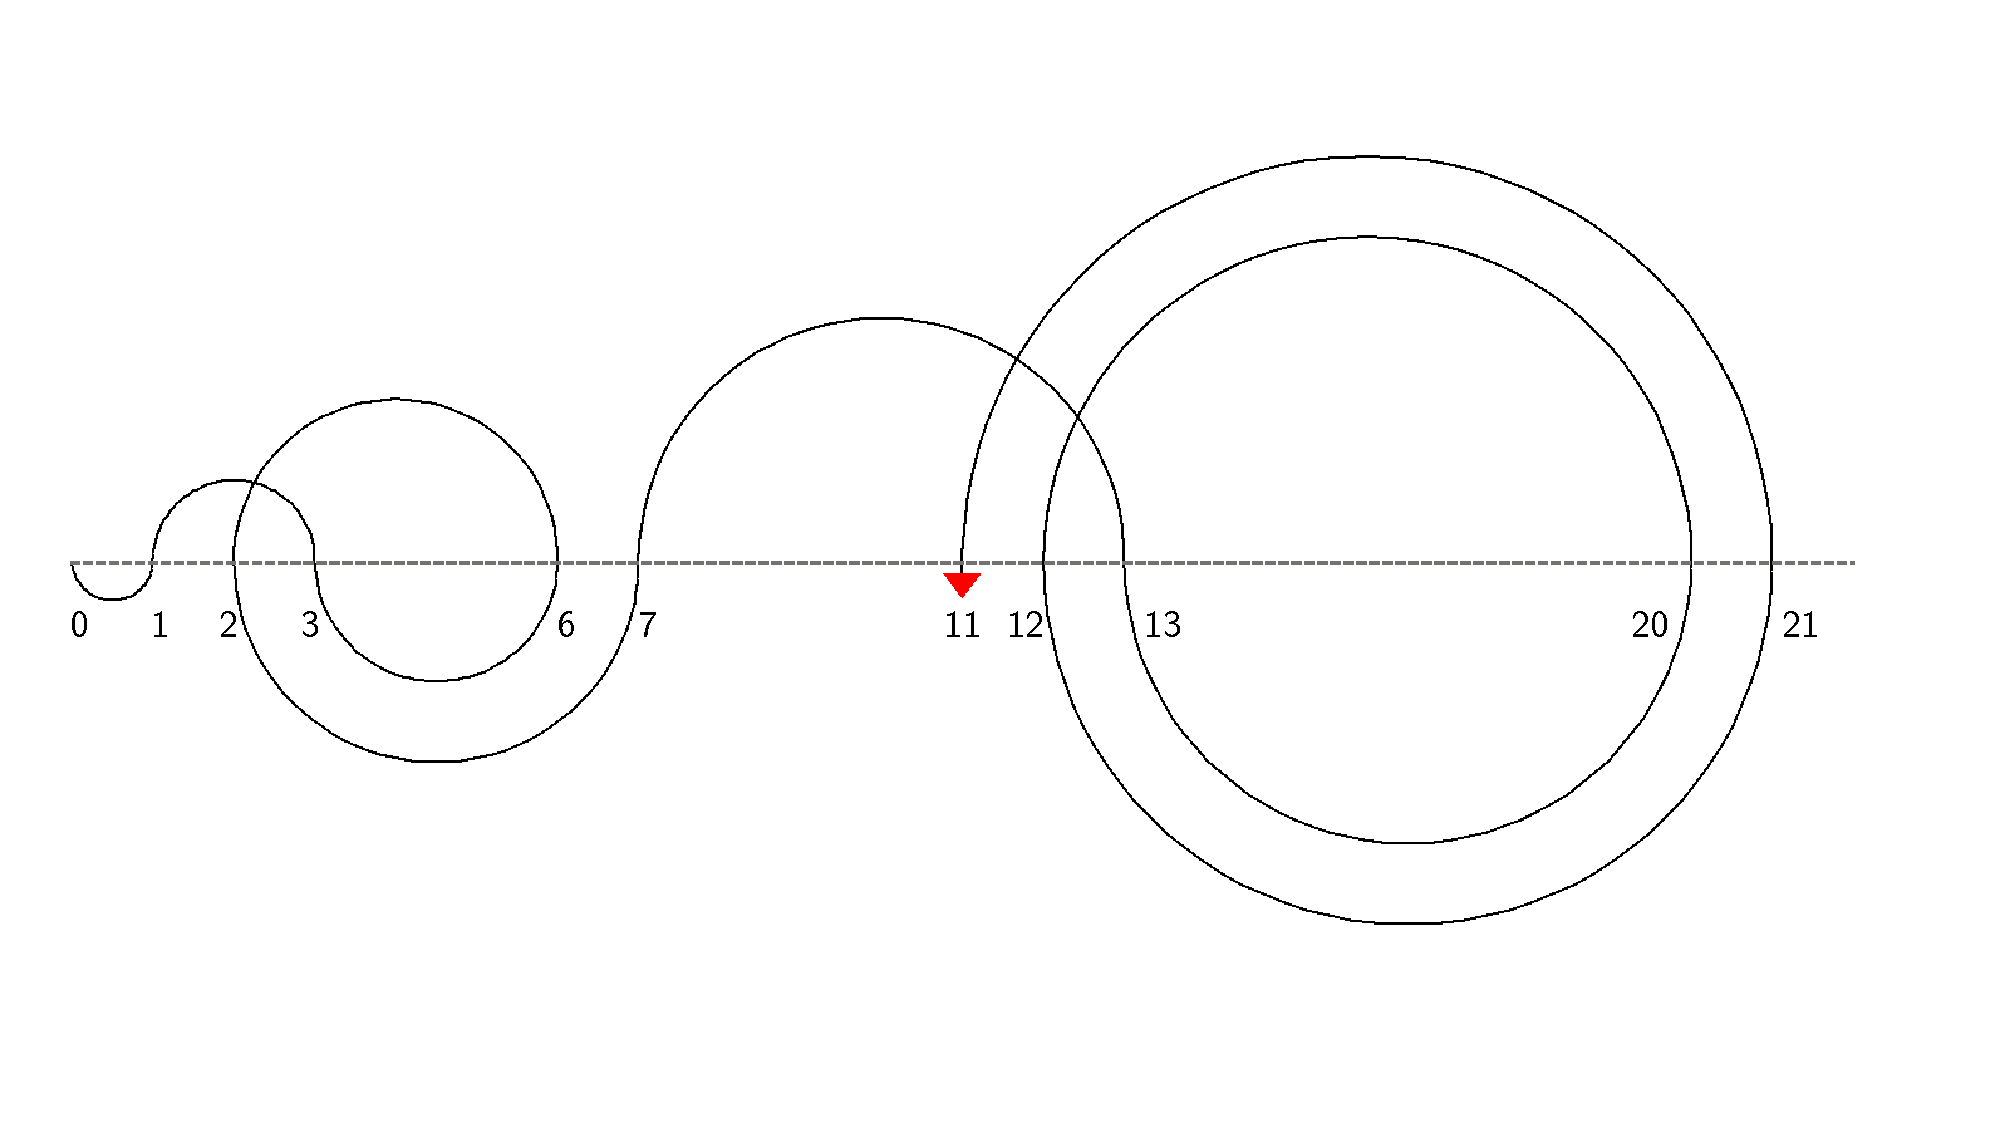
\includegraphics[width=0.7\linewidth]{Recaman's Sequence.pdf}
	\caption{Recaman's Sequence Drawing Procedure}
	\label{fig:recamanssequence}
\end{figure}
\begin{itemize}
\item Create a canvas named ``Recamans Sequence'' with width=1920, and height=1080.
\item Connect all consecutive terms using semicircles.
\item The semicircles should be parallel to $x-$axis with end points as consecutive terms
\item The semicircles should alternate above and below the $x-$axis; i.e., it should be below the axis when connecting $r_0, r_1,$ above the axis when connecting $r_1, r_2,$ again below for $r_2, r_3,$ and so on.
\item The figure should be dynamic; i.e., the $x-$axis should be such that for any $n$ the figure takes up at least half the canvas and it also remains within the canvas.
\item Don't draw the numbers and the axis. They are just to visualise the construction.
\end{itemize}
\textbf{Problem Statement:}\\
Generate the first $n+1$ elements $r_0,r_1,\ldots,r_n$ of the Recaman's Sequence and draw the corresponding curve using \verb!turtleSim!.
\begin{testcasesMore}
	{$n$ \hfill(a single integer)}
	{First $n+1$ elements of the Recaman's sequence and the curve.}
	{$1 \leq n \leq 1000$}
	{60}
	{0 1 3 6 2 7 13 20 12 21 11 22 10 23 9 24 8 25 43 62 42 63 41 18 42 17 43 16 44 15 45 14 46 79 113 78 114 77 39 78 38 79 37 80 36 81 35 82 34 83 33 84 32 85 31 86 30 87 29 88 28}
	{https://github.com/paramrathour/CS-101/tree/main/Test Cases/Recaman's Sequence/Input}
	{https://github.com/paramrathour/CS-101/tree/main/Test Cases/Recaman's Sequence/Output}
	{https://github.com/paramrathour/CS-101/tree/main/Starter Codes/Recaman's Sequence.cpp}
\end{testcasesMore}
\textbf{The output curve}
\begin{figure}[H]
	\centering
	\begin{subfigure}{0.3\linewidth}
		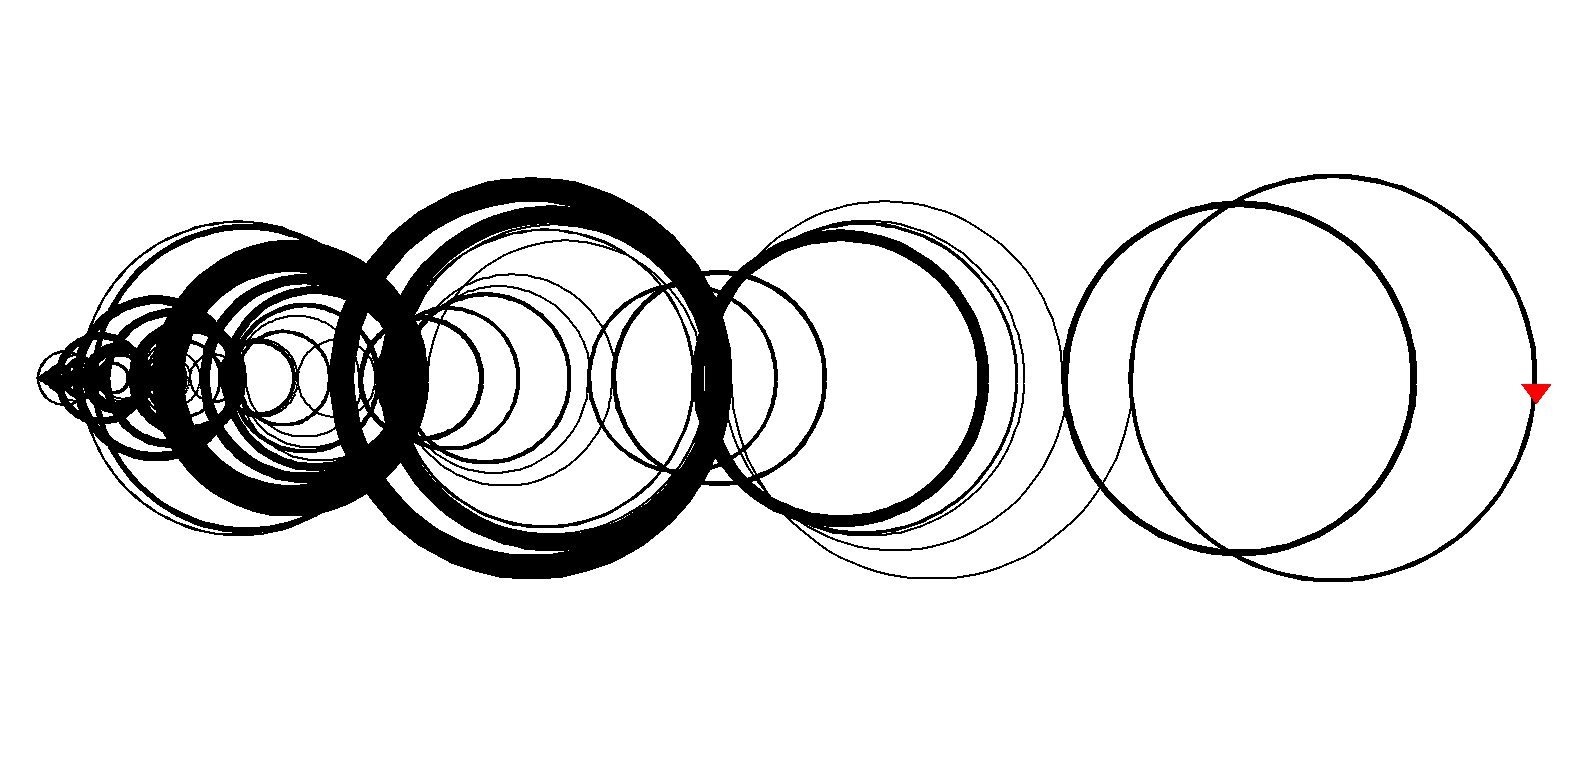
\includegraphics[width = \linewidth]{Recaman's Sequence/10.png}
		\caption{$n=10$}
	\end{subfigure}
	\begin{subfigure}{0.3\linewidth}
		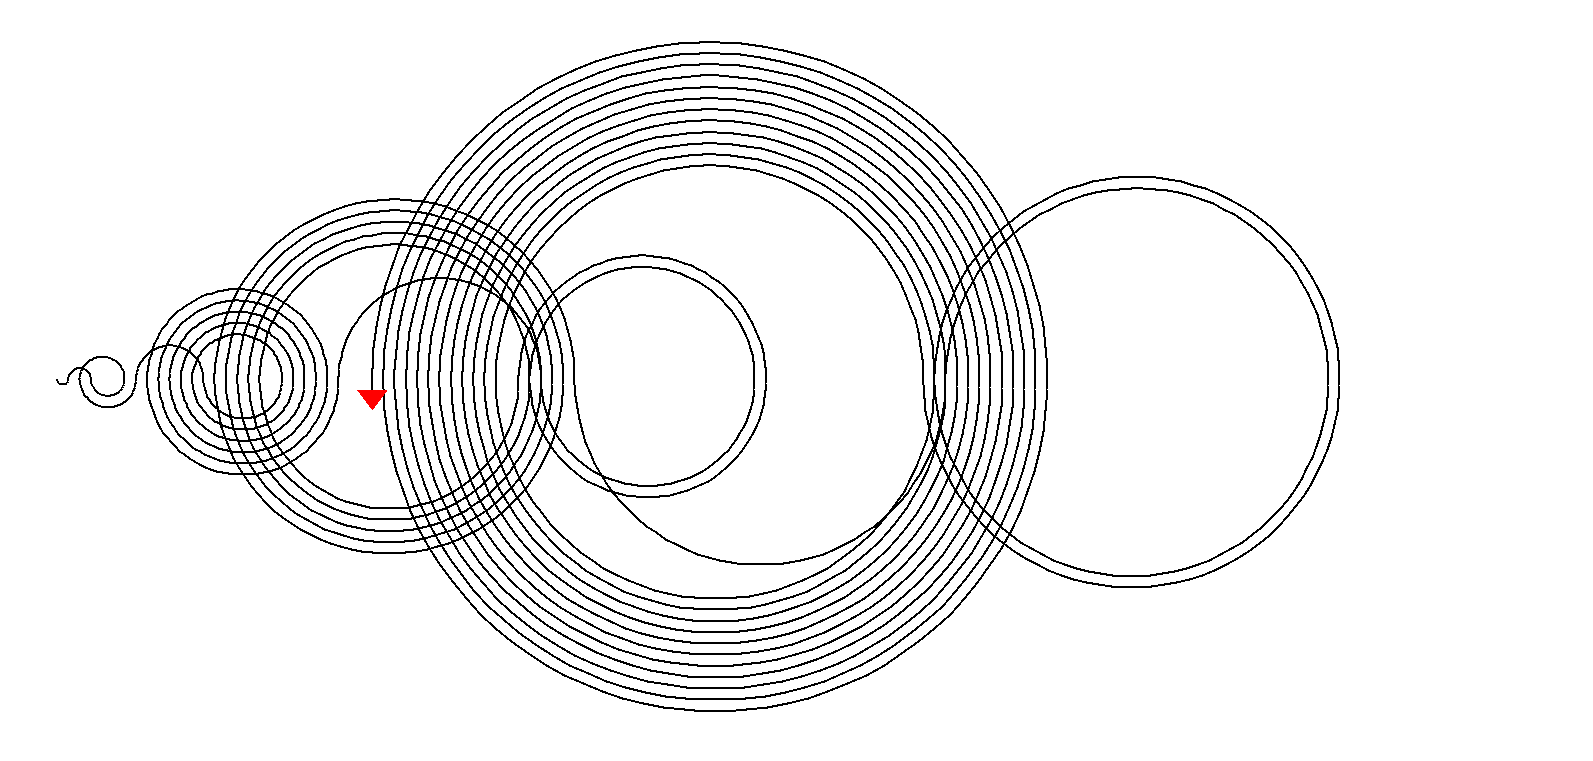
\includegraphics[width = \linewidth]{Recaman's Sequence/60.png}
		\caption{$n=60$}
	\end{subfigure}
	\begin{subfigure}{0.3\linewidth}
		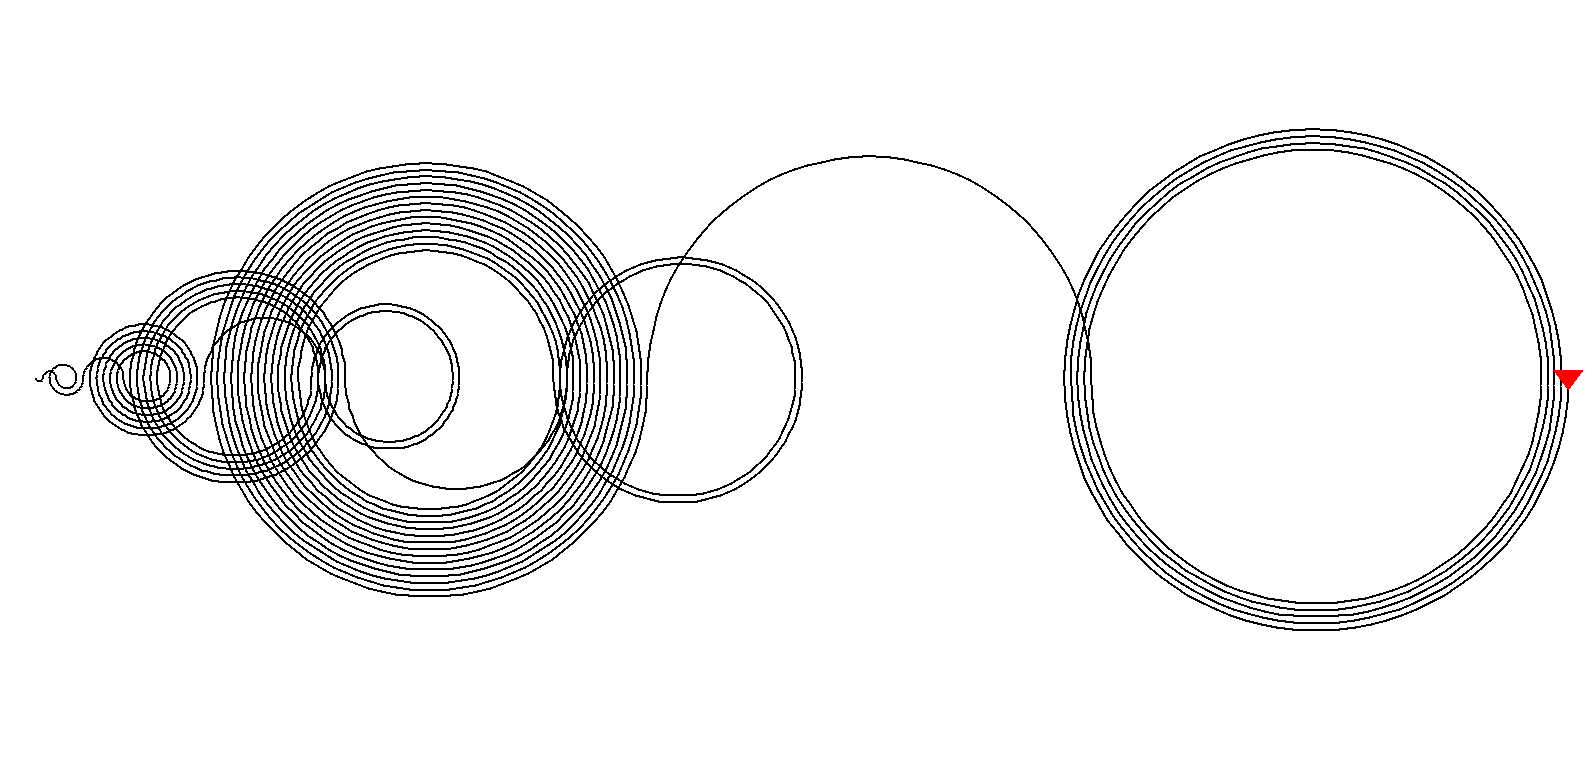
\includegraphics[width = \linewidth]{Recaman's Sequence/75.png}
		\caption{$n=75$}
	\end{subfigure}
	\caption{Output Ford Circles for few $n$}
\end{figure}
\begin{funvideo}
	\href{https://youtu.be/FGC5TdIiT9U}{The Slightly Spooky Recamán Sequence -- Numberphile}
\end{funvideo}
\KOMAoptions{paper=A4}
\recalctypearea